\documentclass[12pt,a4paper]{article}

% ─── Page Layout ───────────────────────────────────────────────────────────────
\usepackage[a4paper, margin=0.8in, headheight=14pt]{geometry}

% ─── Fonts (XeLaTeX) ───────────────────────────────────────────────────────────
\usepackage{fontspec}
\usepackage{unicode-math}
\setmainfont{TeX Gyre Pagella}
\setmonofont[Scale=0.88]{TeX Gyre Cursor}
\setmathfont{Latin Modern Math}

% ─── Packages ──────────────────────────────────────────────────────────────────
\usepackage{xcolor}
\usepackage{colortbl}
\usepackage{titlesec}
\usepackage{enumitem}
\usepackage{tabularx}
\usepackage{booktabs}
\usepackage{array}
\usepackage{amsmath}
\usepackage{tikz}
\usetikzlibrary{shapes.geometric, arrows.meta, positioning, calc, fit, decorations.pathreplacing, patterns}
\usepackage{tcolorbox}
\tcbuselibrary{skins, breakable}
\usepackage{hyperref}
\usepackage{fancyhdr}
\usepackage{graphicx}
\usepackage{microtype}
\hyphenpenalty=10000
\exhyphenpenalty=10000
\sloppy
\usepackage{caption}
\usepackage{setspace}
\usepackage{multirow}
\usepackage{tocloft}

% ─── Q&A helper ────────────────────────────────────────────────────────────────
\newcommand{\Q}[1]{\textbf{#1}\par\noindent\ignorespaces}

% ─── Colour Palette ────────────────────────────────────────────────────────────
\definecolor{myred}{RGB}{196,30,58}
\definecolor{mydark}{RGB}{30,30,50}
\definecolor{mygreen}{RGB}{14,120,80}
\definecolor{myteal}{RGB}{0,130,140}
\definecolor{myamber}{RGB}{180,100,0}
\definecolor{mypurple}{RGB}{100,30,160}
\definecolor{mygray}{RGB}{246,247,249}
\definecolor{mgframe}{RGB}{180,185,200}
\definecolor{watermark}{RGB}{145,150,170}
\definecolor{hdrred}{RGB}{250,232,235}
\definecolor{hdrgreen}{RGB}{220,244,233}
\definecolor{hdrteal}{RGB}{220,242,244}
\definecolor{hdramber}{RGB}{253,242,215}
\definecolor{hdrpurple}{RGB}{238,228,255}
\definecolor{hdrgray}{RGB}{238,240,245}
\definecolor{rowalt}{RGB}{250,251,253}

% ─── Section Formatting ────────────────────────────────────────────────────────
\titleformat{\section}
  {\large\bfseries\color{myred}}{\thesection.}{0.5em}{}
  [\vspace{1pt}{\color{myred}\rule{\linewidth}{0.8pt}}]
\titleformat{\subsection}
  {\normalsize\bfseries\color{myteal}}{\thesubsection}{0.5em}{}
\titlespacing*{\section}{0pt}{18pt}{7pt}
\titlespacing*{\subsection}{0pt}{11pt}{4pt}

% ─── Paragraph ─────────────────────────────────────────────────────────────────
\setlength{\parindent}{0pt}
\setlength{\parskip}{4pt}

% ─── TOC Styling ───────────────────────────────────────────────────────────────
\renewcommand{\cfttoctitlefont}{\large\bfseries\color{myred}}
\renewcommand{\cftaftertoctitle}{\par\noindent{\color{myred}\rule{\linewidth}{0.8pt}}}
\setlength{\cftbeforetoctitleskip}{0pt}
\setlength{\cftaftertoctitleskip}{6pt}
\renewcommand{\cftsecfont}{\normalsize\bfseries\color{mydark}}
\renewcommand{\cftsecpagefont}{\normalsize\bfseries\color{mydark}}
\renewcommand{\cftsecleader}{\cftdotfill{\cftdotsep}}
\setlength{\cftbeforesecskip}{7pt}
\renewcommand{\cftsubsecfont}{\small\color{mydark}}
\renewcommand{\cftsubsecpagefont}{\small\color{mydark}}
\setlength{\cftbeforesubsecskip}{3pt}
\setlength{\cftsubsecindent}{1.4em}

% ─── Table helpers ─────────────────────────────────────────────────────────────
\renewcommand{\arraystretch}{1.45}
\setlength{\tabcolsep}{6pt}
\arrayrulecolor{mydark}
\newcolumntype{B}[1]{>{\small\bfseries\raggedright\arraybackslash}m{#1}}
\newcolumntype{Y}{>{\small\raggedright\arraybackslash}X}
\renewcommand{\tabularxcolumn}[1]{m{#1}}

% ─── Header / Footer ───────────────────────────────────────────────────────────
\pagestyle{fancy}
\fancyhf{}
\fancyhead[L]{\small\color{myred}\textbf{26-ES-EE101}\;\color{mydark}--- Basic Electrical and Electronics Engineering}
\fancyhead[R]{\small\color{myteal}\textbf{Module 4 Notes}}
\fancyfoot[C]{\small\color{mydark}\thepage}
\fancyfoot[R]{\small\color{watermark}\textit{\copyright\ Biraj}}
\renewcommand{\headrulewidth}{0.5pt}
\renewcommand{\footrulewidth}{0.3pt}

% ─── Hyperref ──────────────────────────────────────────────────────────────────
\hypersetup{
  colorlinks=true, linkcolor=myteal, urlcolor=myteal,
  pdfauthor={Biraj Sarkar (CGEC)},
  pdftitle={26-ES-EE101 --- Module 4 Notes: Transformers and Rotating Machines}
}

% ─── tcolorbox styles ──────────────────────────────────────────────────────────
\tcbset{
  tikzbox/.style={
    colback=mygray, colframe=mgframe, boxrule=0.6pt, arc=4pt,
    left=8pt, right=8pt, top=6pt, bottom=6pt,
    colbacktitle=mgframe, coltitle=mydark, fonttitle=\small\bfseries
  },
  defbox/.style={
    colback=hdrgreen, colframe=mygreen, boxrule=0.8pt, arc=4pt,
    left=9pt, right=9pt, top=6pt, bottom=6pt,
    colbacktitle=mygreen, coltitle=white, fonttitle=\small\bfseries
  },
  formulabox/.style={
    colback=hdrteal, colframe=myteal, boxrule=0.8pt, arc=4pt,
    left=9pt, right=9pt, top=7pt, bottom=7pt,
    colbacktitle=myteal, coltitle=white, fonttitle=\small\bfseries
  },
  examplebox/.style={
    colback=hdramber, colframe=myamber, boxrule=0.8pt, arc=4pt,
    left=9pt, right=9pt, top=6pt, bottom=6pt,
    colbacktitle=myamber, coltitle=white, fonttitle=\small\bfseries
  },
  masonbox/.style={
    colback=hdrpurple, colframe=mypurple, boxrule=0.8pt, arc=4pt,
    left=9pt, right=9pt, top=6pt, bottom=6pt,
    colbacktitle=mypurple, coltitle=white, fonttitle=\small\bfseries
  },
  exambox/.style={
    colback=hdrpurple, colframe=mypurple, boxrule=1pt, arc=5pt,
    left=10pt, right=10pt, top=8pt, bottom=8pt,
    colbacktitle=mypurple, coltitle=white, fonttitle=\bfseries,
    breakable, title after break={\textbf{Frequently Asked / Viva Questions (contd.)}}
  }
}
\tcbset{breakable}
\tcbset{after={\par\color{black}}}

% ─── TikZ styles ───────────────────────────────────────────────────────────────
\tikzset{
  block/.style={rectangle, draw=myteal, fill=hdrteal,
    text width=2.4cm, align=center, minimum height=0.95cm,
    font=\small, rounded corners=3pt, line width=0.7pt},
  redblock/.style={rectangle, draw=myred, fill=hdrred,
    text width=2.4cm, align=center, minimum height=0.95cm,
    font=\small, rounded corners=3pt, line width=0.7pt},
  sumjunc/.style={circle, draw=myamber, fill=hdramber,
    minimum size=0.62cm, font=\small, line width=0.8pt},
  arrow/.style={-Stealth, thick, color=mydark},
  redarrow/.style={-Stealth, thick, color=myred},
  line/.style={thick, color=mydark}
}

\begin{document}

% ─── Title Page ───────────────────────────────────────────────────────────────
\begin{center}
  {\Large\bfseries\color{myred} 26-ES-EE101}\\[3pt]
  {\LARGE\bfseries\color{myred} Basic Electrical and Electronics Engineering}\\[5pt]
  {\normalsize\color{mydark} Semester I \quad$\bullet$\quad 3L:1T:0P \quad$\bullet$\quad 4 Credits}\\[3pt]
  {\normalsize\color{myteal}\textbf{Module 4 Exam Notes: Transformers and Rotating Machines}}\\[3pt]
  {\small\color{mydark} CGEC \;$|$\; MAKAUT Syllabus (A.Y. 2026--27) \;$|$\; \textit{Biraj Sarkar}}
\end{center}
\vspace{2pt}
\noindent{\color{myred}\rule{\linewidth}{1.5pt}}
\vspace{2pt}

\hypersetup{linkcolor=mydark}
\tableofcontents
\hypersetup{linkcolor=myteal}
\newpage

\section{Transformers and Rotating Machines}

\subsection{Single-phase transformer}
\begin{tcolorbox}[defbox,title={Transformer and mutual induction}]
A transformer is a static AC device that transfers electrical energy between windings through a common changing magnetic flux. Frequency remains the same. Mutual induction is the production of an emf in one winding by changing flux produced by another.
\end{tcolorbox}

\begin{itemize}[leftmargin=*, itemsep=3pt, topsep=4pt]
  \item \textbf{Construction.} Insulated primary and secondary windings share a laminated steel core. Laminations limit eddy currents. Common arrangements are core type and shell type.
  \item \textbf{At no load.} AC in the primary establishes alternating core flux and induces emf in both windings.
  \item \textbf{With a load.} Secondary current causes the primary to draw an additional current. The additional primary and secondary ampere-turns approximately balance.
  \item \textbf{With steady DC.} After switching, the flux no longer changes. There is no sustained secondary emf, and primary current can become excessive.
\end{itemize}

\begin{tcolorbox}[tikzbox,title={Windings and shared magnetic flux},unbreakable]
\centering
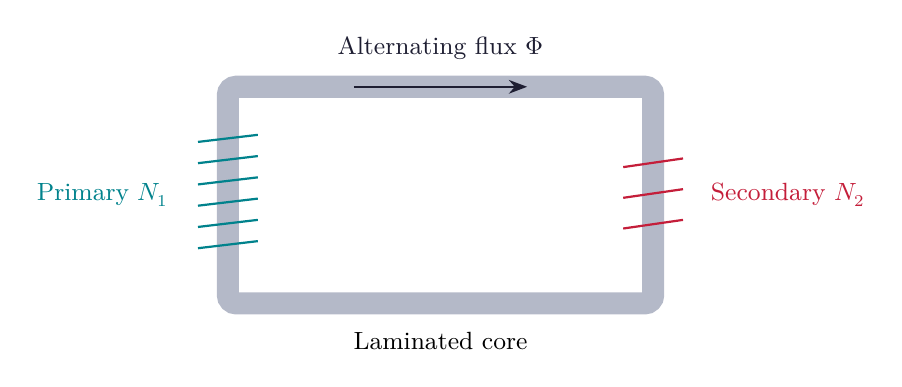
\begin{tikzpicture}[font=\small]
\draw[mgframe,line width=8pt,rounded corners=3pt] (0,0) rectangle (5.4,2.75);
\draw[-Stealth,mydark,thick] (1.6,2.75)--(3.8,2.75) node[midway,above=6pt] {Alternating flux $\Phi$};
\foreach \y in {0.7,0.97,1.24,1.51,1.78,2.05} {
  \draw[myteal,thick] (-0.38,\y)--(0.38,\y+0.09);
}
\foreach \y in {0.95,1.34,1.73} {
  \draw[myred,thick] (5.02,\y)--(5.78,\y+0.11);
}
\node[myteal,left=6pt] at (-0.42,1.38) {Primary $N_1$};
\node[myred,right=6pt] at (5.8,1.38) {Secondary $N_2$};
\node[below=7pt] at (2.7,0) {Laminated core};
\end{tikzpicture}
\end{tcolorbox}

For sinusoidal flux \(\Phi=\Phi_m\sin\omega t\), Faraday's law gives peak emf \(\omega N\Phi_m\). Hence
\[
\begin{aligned}
E_{\mathrm{rms}}&=\frac{2\pi fN\Phi_m}{\sqrt 2}\\
                &\approx 4.44 fN\Phi_m .
\end{aligned}
\]
Use \(f\) in hertz and peak flux in webers. For the ideal transformer, with \(a=N_1/N_2\), the magnitudes satisfy \(V_1/V_2=a\) and \(I_1/I_2=1/a\). An impedance on the secondary is referred to the primary as \(Z'_2=a^2Z_2\). Derive this by using \(V'_2=aV_2\) and \(I'_2=I_2/a\) in the impedance ratio.

\subsection{Equivalent circuit, losses and performance}
\begin{itemize}[leftmargin=*, itemsep=3pt, topsep=4pt]
  \item \textbf{Series elements.} Each winding has a resistance \(R_1\) or \(R_2\) for copper loss and a leakage reactance \(X_1\) or \(X_2\) for flux that links only that winding.
  \item \textbf{Shunt elements.} Across the induced primary emf, \(R_c\) represents core loss and \(jX_m\) represents the magnetising current.
  \item \textbf{Refer to the primary.} Multiply secondary impedance by \(a^2\), where \(a=N_1/N_2\). Hence \(R_{\mathrm{eq}}=R_1+a^2R_2\) and \(X_{\mathrm{eq}}=X_1+a^2X_2\).
  \item \textbf{Approximate circuit.} Move the shunt branch to the supply terminals. This neglects the small primary series drop due to no-load current.
\end{itemize}

\begin{tcolorbox}[tikzbox,title={Approximate equivalent circuit referred to the primary},unbreakable]
\centering
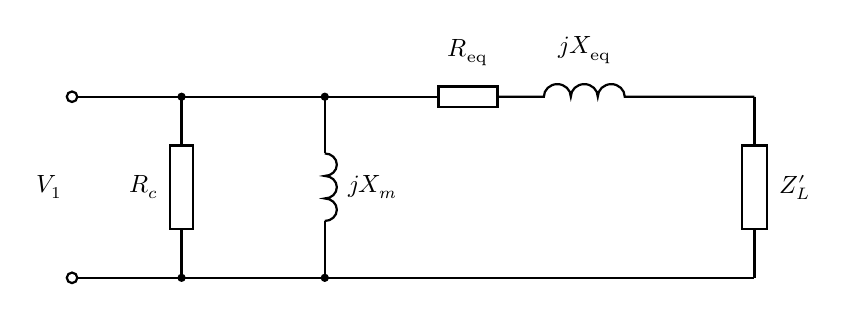
\begin{tikzpicture}[x=1.07cm,font=\small]
\draw[thick] (0,2.3)--(5.05,2.3) (0,0)--(8.1,0);
\draw[thick] (1.3,2.3)--(1.3,1.68) (1.3,0.62)--(1.3,0);
\draw[thick,fill=white] (1.16,0.62) rectangle (1.44,1.68);
\node[left] at (1.14,1.15) {$R_c$};
\draw[thick] (3.0,2.3)--(3.0,1.58) (3.0,0.72)--(3.0,0);
\draw[thick] (3.0,1.58) arc[start angle=90,end angle=-90,radius=0.143]
 arc[start angle=90,end angle=-90,radius=0.143]
 arc[start angle=90,end angle=-90,radius=0.143];
\node[right] at (3.16,1.15) {$jX_m$};
\draw[thick,fill=white] (4.35,2.17) rectangle (5.05,2.43);
\node[above=4pt] at (4.70,2.43) {$R_{\mathrm{eq}}$};
\draw[thick] (5.05,2.3)--(5.60,2.3)
 arc[start angle=180,end angle=0,radius=0.16]
 arc[start angle=180,end angle=0,radius=0.16]
 arc[start angle=180,end angle=0,radius=0.16] -- (8.1,2.3);
\node[above=4pt] at (6.09,2.46) {$jX_{\mathrm{eq}}$};
\draw[thick] (8.1,2.3)--(8.1,1.68) (8.1,0.62)--(8.1,0);
\draw[thick,fill=white] (7.95,0.62) rectangle (8.25,1.68);
\node[right] at (8.28,1.15) {$Z'_L$};
\node[left] at (0,1.15) {$V_1$};
\foreach \x in {1.3,3.0} {\fill (\x,2.3) circle (1.5pt); \fill (\x,0) circle (1.5pt);}
\draw[thick,fill=white] (0,0) circle (1.9pt) (0,2.3) circle (1.9pt);
\end{tikzpicture}
\end{tcolorbox}

\textbf{Losses to identify.}
\begin{itemize}[leftmargin=*, itemsep=3pt, topsep=4pt]
  \item \textbf{Core loss.} Hysteresis and eddy-current losses. Approximately constant at fixed supply voltage and frequency.
  \item \textbf{Copper loss.} \(I_1^2R_1+I_2^2R_2\). At load fraction \(x\), approximate it as \(x^2P_{\mathrm{cu,full}}\).
  \item \textbf{Other losses.} Stray load and dielectric losses also occur. The basic efficiency model below uses core and copper losses.
\end{itemize}

\textbf{Efficiency.} For a rating \(S_r\) in VA and load power factor \(\cos\phi\), output power is \(xS_r\cos\phi\) in W.
\[
\eta=\frac{xS_r\cos\phi}{xS_r\cos\phi+P_{\mathrm{core}}+x^2P_{\mathrm{cu,full}}}.
\]
Multiply \(\eta\) by 100 for percentage efficiency. At fixed positive power factor, maximising \(\eta\) is equivalent to minimising loss per unit of output. Apart from the constant \(1/(S_r\cos\phi)\), this gives
\[
\begin{aligned}
g(x)&=\frac{P_{\mathrm{core}}}{x}+xP_{\mathrm{cu,full}},\\
g'(x)&=-\frac{P_{\mathrm{core}}}{x^2}+P_{\mathrm{cu,full}},\\
g'(x)=0 &\quad\Longrightarrow\quad x^2P_{\mathrm{cu,full}}=P_{\mathrm{core}}.
\end{aligned}
\]
This is a minimum for \(x>0\) since \(g''(x)=2P_{\mathrm{core}}/x^3>0\). \textbf{Exam point.} At the optimum, the copper loss at that load equals the core loss.

Voltage regulation is the change in secondary terminal voltage from full load to no load with primary voltage held constant, divided by the full-load secondary voltage:
\[
\%\,\mathrm{reg}=\frac{V_{2,\mathrm{nl}}-V_{2,\mathrm{fl}}}{V_{2,\mathrm{fl}}}\times100 .
\]
\begin{itemize}[leftmargin=*, itemsep=3pt, topsep=4pt]
  \item \textbf{Lagging load.} For small voltage drops, approximate the numerator by \(I_2(R_{\mathrm{eq,2}}\cos\phi+X_{\mathrm{eq,2}}\sin\phi)\). All impedances here are referred to the secondary.
  \item \textbf{Leading load.} Use a minus sign for the reactance term. The no-load voltage can then be lower than the loaded voltage, giving negative regulation.
\end{itemize}

\begin{tcolorbox}[examplebox,title={Transformer performance at partial load}]
For a \(5\,\mathrm{kVA}\) transformer with \(60\,\mathrm W\) core loss and \(240\,\mathrm W\) full-load copper loss, take \(x=0.5\), \(\cos\phi=0.8\):
\[
\begin{aligned}
P_o&=(0.5)(5000)(0.8)=2000\,\mathrm W,\\
P_{\mathrm{cu}}&=(0.5)^2(240)=60\,\mathrm W,\\
\eta&=\frac{2000}{2000+60+60}=94.34\%.
\end{aligned}
\]
The core and copper losses are equal here, so this load fraction gives maximum efficiency at the same power factor.
\end{tcolorbox}

An \textbf{autotransformer} uses a tapped winding with a portion common to input and output. It transfers energy partly by conduction and partly by induction. For a ratio near unity it can save copper and reduce losses. The shared winding provides no galvanic isolation. Applications include voltage adjustment and reduced-voltage motor starting.

\subsection{DC machine construction and equations}
\begin{itemize}[leftmargin=*, itemsep=3pt, topsep=4pt]
  \item \textbf{Field system.} The stationary yoke and poles carry magnetic flux. Field windings or permanent magnets supply the excitation.
  \item \textbf{Armature.} A laminated rotor houses conductors in slots. The commutator connects the rotating conductors to stationary brushes.
  \item \textbf{Generator action.} The commutator switches coil connections so the voltage at the brushes is unidirectional.
  \item \textbf{Motor action.} As a coil crosses from one pole region to another, the commutator reverses its current to maintain the direction of torque.
\end{itemize}

For \(P\) poles, flux \(\Phi\) per pole in Wb, \(Z\) armature conductors, \(A\) parallel paths and speed \(N\) in rpm,
\[
\begin{aligned}
\text{flux swept per conductor per revolution}&=P\Phi,\\
\text{revolution time}&=60/N,\\
E&=\frac{P\Phi N}{60}\frac{Z}{A}.
\end{aligned}
\]
Neglect brush drop for the basic terminal equations:
\[
\begin{aligned}
V&=E-I_aR_a &&\text{generator supplying current},\\
V&=E_b+I_aR_a &&\text{motor drawing current}.
\end{aligned}
\]
In the motor, back emf \(E_b\) opposes the applied voltage. Divide the electromagnetic conversion power \(E_b I_a\) by \(\omega_m=2\pi N/60\) in rad/s to find torque.
\[
\begin{aligned}
T_e&=\frac{E_b I_a}{\omega_m}\\
   &=\frac{PZ}{2\pi A}\Phi I_a \quad(\mathrm{N\,m}).
\end{aligned}
\]
Shaft torque equals electromagnetic torque less the rotational-loss torque in motor operation.

\par\vspace{6pt}\noindent
\begin{tabularx}{\linewidth}{|B{3.4cm}|Y|Y|}\hline
Excitation & \textbf{Connection} & \textbf{Motor characteristic} \\ \hline
Separately excited & Field supplied externally. & Field and armature can be adjusted independently. \\ \hline
Shunt & Field across terminal supply. & Flux approximately constant, so speed changes moderately and torque is approximately proportional to \(I_a\). \\ \hline
Series & Field carries armature current. & Large starting torque, with torque approximately proportional to \(I_a^2\) before saturation. Speed can run high at light load. \\ \hline
Compound & Both shunt and series fields. & Cumulative compounding adds the two field effects and combines starting torque with better speed control than a series motor. \\ \hline
\end{tabularx}

\begin{itemize}[leftmargin=*, itemsep=3pt, topsep=4pt]
  \item \textbf{Shunt generator.} Terminal voltage droops under load because of the armature voltage drop and field and armature effects.
  \item \textbf{Series generator.} Voltage initially rises with load current. Magnetic saturation and internal drops limit that rise.
  \item \textbf{Compound generator.} Cumulative compounding adds series-field flux and can compensate terminal-voltage drop. Differential compounding subtracts series-field flux.
  \item \textbf{Motor speed.} For a given machine, \(N\) varies approximately as \((V-I_aR_a)/\Phi\). A series motor can overspeed at light load.
  \item \textbf{Starting.} At standstill \(N=0\) and \(E_b=0\), so the armature current would be high. A starter limits it using series resistance cut out in steps or electronic current limiting.
\end{itemize}

\begin{tcolorbox}[examplebox,title={DC motor back emf and converted torque}]
For \(V=220\,\mathrm V\), \(R_a=0.5\,\Omega\), \(I_a=20\,\mathrm A\) and \(N=1000\,\mathrm{rpm}\),
\[
\begin{aligned}
E_b&=220-(20)(0.5)=210\,\mathrm V,\\
P_{\mathrm{conv}}&=(210)(20)=4200\,\mathrm W,\\
T_e&=\frac{4200}{2\pi(1000)/60}=40.1\,\mathrm{N\,m}.
\end{aligned}
\]
\end{tcolorbox}

\subsection{AC motors, stepper motors and BLDC motors}
\begin{itemize}[leftmargin=*, itemsep=3pt, topsep=4pt]
  \item \textbf{Rotating field.} A balanced three-phase stator produces a field at \(N_s=120f/P\) rpm, with \(P\) poles and frequency \(f\) in Hz.
  \item \textbf{Induction motor.} Relative motion induces rotor current. That current interacts with the field to produce torque. A squirrel-cage rotor uses bars and end rings. A wound rotor can connect to external resistance through slip rings.
  \item \textbf{Synchronous motor.} The rotor field locks to the rotating stator field, so steady speed is \(N_s\).
\end{itemize}

In an induction motor, slip is \(s=(N_s-N_r)/N_s\), where \(N_r\) is rotor speed. Rotor electrical frequency is \(sf\). For a four-pole motor with \(f=50\,\mathrm{Hz}\) and \(N_r=1440\,\mathrm{rpm}\),
\[
\begin{aligned}
N_s &=120(50)/4=1500\,\mathrm{rpm},\\
s   &=(1500-1440)/1500=0.04,\\
sf  &=(0.04)(50)=2\,\mathrm{Hz}.
\end{aligned}
\]

\begin{tcolorbox}[tikzbox,title={From rotating field to induction-motor torque},unbreakable]
\centering
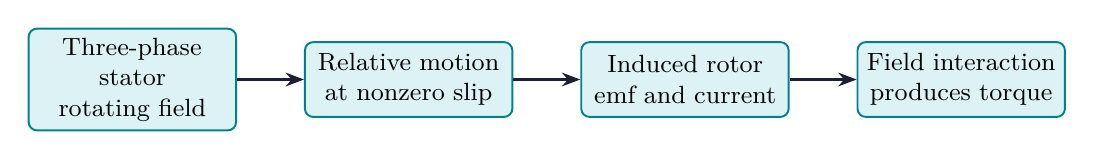
\begin{tikzpicture}[node distance=0.85cm,font=\small]
\node[block] (field) {Three-phase stator\\rotating field};
\node[block,right=of field] (slip) {Relative motion\\at nonzero slip};
\node[block,right=of slip] (current) {Induced rotor\\emf and current};
\node[block,right=of current] (torque) {Field interaction\\produces torque};
\draw[arrow] (field)--(slip);
\draw[arrow] (slip)--(current);
\draw[arrow] (current)--(torque);
\end{tikzpicture}
\end{tcolorbox}

\begin{itemize}[leftmargin=*, itemsep=3pt, topsep=4pt]
  \item \textbf{Main winding alone.} The pulsating field is equivalent to equal forward and backward rotating fields. Opposite torques cancel at standstill.
  \item \textbf{Starting methods.} Split-phase, capacitor-start and shaded-pole arrangements create a starting field asymmetry.
  \item \textbf{Applications.} Fans, pumps and domestic equipment.
\end{itemize}

\begin{itemize}[leftmargin=*, itemsep=3pt, topsep=4pt]
  \item \textbf{Stepper motor.} Sequential phase excitation advances the rotor in steps. A \(1.8^\circ\) motor takes \(360/1.8=200\) full steps per revolution. Indexing can use open-loop control within torque and speed limits. Feedback helps detect missed steps.
  \item \textbf{Brushless DC motor (BLDC).} A permanent-magnet rotor runs inside electronically commutated stator windings. The controller uses position sensing or sensorless estimation to switch phases. In automation, BLDC motors drive pumps, fans and servo axes.
\end{itemize}

\newpage
\begin{center}
  {\large\bfseries\color{myred} Quick Revision --- Module 4}\\[3pt]
  {\small\color{mydark} Transformers and Rotating Machines $|$ 26-ES-EE101}
\end{center}
\noindent{\color{myred}\rule{\linewidth}{1.2pt}}
\vspace{4pt}

\begin{tcolorbox}[formulabox, title={Key Formulas and Concepts at a Glance}]
\renewcommand{\arraystretch}{1.35}
\begin{tabularx}{\linewidth}{B{4.4cm}Y}
Transformer emf & $E=4.44fN\Phi_m$ in V for sinusoidal flux. \\[3pt]
Ideal turns ratio & $V_1/V_2=a$, $I_1/I_2=1/a$, $Z'_2=a^2Z_2$. \\[3pt]
DC emf and torque & $E=P\Phi ZN/(60A)$; $T_e=(PZ/2\pi A)\Phi I_a$. \\[3pt]
Speed and slip & $N_s=120f/P$ in rpm; $s=(N_s-N_r)/N_s$. \\[3pt]
\end{tabularx}
\end{tcolorbox}

\begin{tcolorbox}[defbox, title={One-Line Definitions}]
\textbf{Voltage regulation.} No-load to full-load voltage drop as a percentage of full-load voltage.

\textbf{Back emf.} Armature emf that opposes the applied voltage in a motor.

\textbf{Electronic commutation.} Timed switching of stator phases using a drive circuit.
\end{tcolorbox}

\begin{tcolorbox}[exambox, title={Frequently Asked / Viva Questions}]
\begin{enumerate}[topsep=0pt, label=\textbf{Q\arabic*.}, itemsep=5pt]
  \item \Q{Why laminate the core?} To limit circulating eddy currents and their losses.
  \item \Q{Why does transformer frequency stay the same?} The same alternating flux links the windings.
  \item \Q{What does the magnetising branch represent?} Core loss and current needed to establish flux.
  \item \Q{When is transformer efficiency maximum?} In the simple model at fixed power factor, when copper loss equals core loss.
  \item \Q{What is a main limitation of an autotransformer?} Its input and output are electrically connected through the common winding.
  \item \Q{What is the purpose of a motor starter?} It limits the large initial armature current while back emf is low.
  \item \Q{How does a series DC motor develop high starting torque?} Before saturation the flux rises with armature current, so torque is roughly proportional to $I_a^2$.
  \item \Q{Why is slip needed in an induction motor?} Relative motion induces rotor emf and develops torque.
  \item \Q{Why does a single-phase induction motor need a starting arrangement?} Its two opposing field components produce zero net starting torque with the main winding alone.
  \item \Q{How does a BLDC motor commutate?} An electronic controller switches the stator phases in sequence.
\end{enumerate}
\end{tcolorbox}

\begin{tcolorbox}[tikzbox, title={Summary Reference}]
\begin{tabularx}{\linewidth}{|B{4.0cm}|Y|}\hline
Topic & \textbf{What to remember} \\ \hline
Transformer & Static magnetic energy transfer with voltage conversion. \\ \hline
DC motor & Mechanical commutator and brushes switch armature current. \\ \hline
Induction motor & Rotor currents are induced by relative motion. \\ \hline
Stepper / BLDC & Discrete positioning / electronically commutated rotation. \\ \hline
\end{tabularx}
\end{tcolorbox}

\end{document}

